\documentclass{standalone}

\usepackage{tikz}
\usepackage{xcolor}
\usepackage{amsmath}
\usepackage{nicefrac}

\definecolor{jet}{HTML}{363636}
\definecolor{outerspace}{HTML}{464646}
\definecolor{granitegray}{HTML}{616161}
\definecolor{raisinblack}{HTML}{252525}
\definecolor{tigerseye}{HTML}{EB9438}
\definecolor{denimblue}{HTML}{2B3EAB}
\definecolor{englishgreen}{HTML}{26523C}
\definecolor{upmaroon}{HTML}{780D14}
\definecolor{isabelline}{HTML}{EDEDED}
\definecolor{palmleaf}{HTML}{6DA63F}

\usetikzlibrary{shapes.arrows,chains,calc,decorations.pathreplacing}
\newcommand{\I}{\color{isabelline}}
\newcommand{\N}{{\color{tigerseye} n}\I}
\newcommand{\C}{\color{palmleaf}}
\def\centerarc[#1](#2)(#3:#4:#5)% Syntax: [draw options] (center) (initial angle:final angle:radius)
{ \draw[#1] ($(#2)+({#5*cos(#3)},{#5*sin(#3)})$) arc (#3:#4:#5); }

\begin{document}

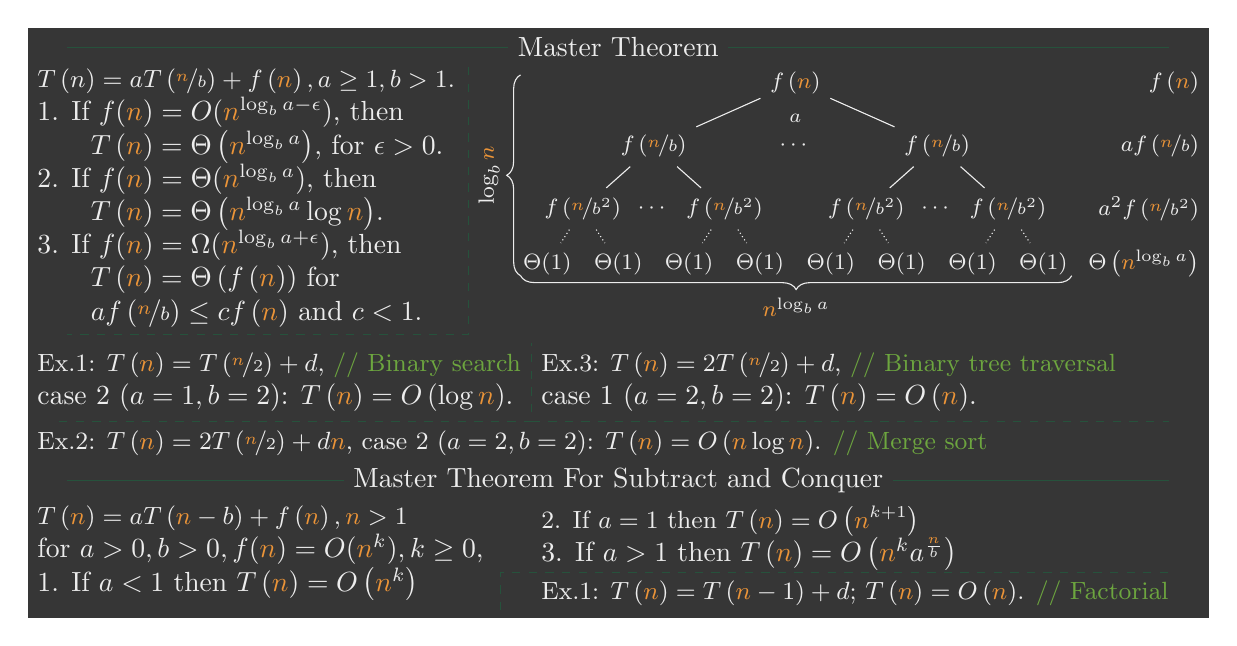
\begin{tikzpicture}
  % Background
  \fill [jet] (0, -2.5) rectangle (15, 5);

  % Block name
  \node at(7.5, 4.75) (mastermethod) {\I Master Theorem};
  \draw[englishgreen] (0.5,4.75) -- (mastermethod.west); 
  \draw[englishgreen] (mastermethod.east) -- (14.5, 4.75);

  \node[align=left] at(0, 4.6)[anchor=north west] {
    \small
    $\I T\left(n\right)=aT\left(\nicefrac{\N}{b}\right) + f\left(\N\right), a \ge 1, b > 1.$\\
    \I 1. If $f(\N)=O(\N^{\log_{b} a - \epsilon})$, then \\
    \I \hspace{5.6mm} $T\left(\N\right) = \Theta\left(\N^{\log_{b} a}\right)$, for $\epsilon>0$.\\
    \I 2. If $f(\N)=\Theta(\N^{\log_{b} a})$, then \\
    \I \hspace{5.6mm} $T\left(\N\right) = \Theta\left(\N^{\log_{b} a}\log \N\right)$.\\
    \I 3. If $f(\N)=\Omega(\N^{\log_{b} a + \epsilon})$, then \\
    \I \hspace{5.6mm} $T\left(\N\right) = \Theta\left(f\left(\N\right)\right)$ for\\
    \I \hspace{5.6mm} $af\left(\nicefrac{\N}{b}\right) \le cf\left(\N\right)$ and $c<1$.\\
  };

  \draw[englishgreen,dashed] (5.6, 4.5) -- (5.6,1.1) -- (0.5, 1.1); 

  \node[align=left] at(0, 1.0)[anchor=north west] {
    \small \I Ex.1:
    \I $T\left(\N \right)=T\left(\nicefrac{\N}{2}\right) + d$,  \C // Binary search \\
    \I case 2 $(a=1,b=2)$: $T\left(\N\right)=O\left(\log \N\right)$.
  };

  \node[align=left] at(0, 0.0)[anchor=north west] {
    \small \I Ex.2:
    \I $T\left(\N \right)=2T\left(\nicefrac{\N}{2}\right) + d\N$,
    \I case 2 $(a=2,b=2)$: $T\left(\N\right)=O\left(\N\log\N\right)$. \C // Merge sort
  };

  \draw[englishgreen,dashed] (0.4, 0.0) -- (6.4,0.0) -- (6.4, 1.0); 
  \draw[englishgreen,dashed] (6.4,0.0) -- (14.5, 0.0); 

  \node[align=left] at(6.4, 1.0)[anchor=north west] {
    \small \I Ex.3:
    \I $T\left(\N \right)=2T\left(\nicefrac{\N}{2}\right) + d$,  \C // Binary tree traversal\\
    \I case 1 $(a=2,b=2)$: $T\left(\N\right)=O\left(\N\right)$.
  };

  % Scheme begin
  % Root
  \node at(9.75,4.3) (root)  {\footnotesize\I$f\left(\N\right)$};

  % Level 1
  \node at(7.95,3.5)[anchor=center] (l1s1)  {\footnotesize\I$f\left(\nicefrac{\N}{b}\right)$};
  \node at(9.75,3.5)[anchor=center]         {\footnotesize\I$\cdots$};
  \node at(11.55,3.5)[anchor=center] (l1s3) {\footnotesize\I$f\left(\nicefrac{\N}{b}\right)$};
  \node at(9.75,3.85)[anchor=center]        {\scriptsize\I$a$};
  \draw[isabelline] (root) -- (l1s1);
  \draw[isabelline] (root) -- (l1s3);
  \centerarc[isabelline,dashed](9.75,5.9)(250:290:2.2)

  % Level 2
  \node at(7.05,2.7)[anchor=center] (l2p1s1)  {\footnotesize\I$f\left(\nicefrac{\N}{b^2}\right)$};
  \node at(7.95,2.7)[anchor=center]           {\footnotesize\I$\cdots$};
  \node at(8.85,2.7)[anchor=center] (l2p1s3)  {\footnotesize\I$f\left(\nicefrac{\N}{b^2}\right)$};
  \draw[isabelline] (l1s1) -- (l2p1s1);
  \draw[isabelline] (l1s1) -- (l2p1s3);
  \centerarc[isabelline,dashed](7.95,5.25)(260:280:2.2)

  \node at(10.65,2.7)[anchor=center] (l2p3s1)  {\footnotesize\I$f\left(\nicefrac{\N}{b^2}\right)$};
  \node at(11.55,2.7)[anchor=center]           {\footnotesize\I$\cdots$};
  \node at(12.45,2.7)[anchor=center] (l2p3s3)  {\footnotesize\I$f\left(\nicefrac{\N}{b^2}\right)$};
  \draw[isabelline] (l1s3) -- (l2p3s1);
  \draw[isabelline] (l1s3) -- (l2p3s3);
  \centerarc[isabelline,dashed](11.55,5.25)(260:280:2.2)

  % Level 3
  \node at(6.6,2)[anchor=center] (l3p1s1)  {\footnotesize\I$\Theta(1)$};
  \node at(7.5,2)[anchor=center] (l3p1s3)  {\footnotesize\I$\Theta(1)$};
  \draw[isabelline,densely dotted] (l2p1s1) -- (l3p1s1);
  \draw[isabelline,densely dotted] (l2p1s1) -- (l3p1s3);

  \node at(8.4,2)[anchor=center] (l3p3s1)  {\footnotesize\I$\Theta(1)$};
  \node at(9.3,2)[anchor=center] (l3p3s3)  {\footnotesize\I$\Theta(1)$};
  \draw[isabelline,densely dotted] (l2p1s3) -- (l3p3s1);
  \draw[isabelline,densely dotted] (l2p1s3) -- (l3p3s3);
  
  \node at(10.2,2)[anchor=center] (l3p4s1)  {\footnotesize\I$\Theta(1)$};
  \node at(11.1,2)[anchor=center] (l3p4s3)  {\footnotesize\I$\Theta(1)$};
  \draw[isabelline,densely dotted] (l2p3s1) -- (l3p4s1);
  \draw[isabelline,densely dotted] (l2p3s1) -- (l3p4s3);

  \node at(12.0,2)[anchor=center] (l3p5s1)  {\footnotesize\I$\Theta(1)$};
  \node at(12.9,2)[anchor=center] (l3p5s3)  {\footnotesize\I$\Theta(1)$};
  \draw[isabelline,densely dotted] (l2p3s3) -- (l3p5s1);
  \draw[isabelline,densely dotted] (l2p3s3) -- (l3p5s3);

  \node[align=center] at(15,4.3)[anchor=east] {\footnotesize\I$f\left(\N\right)$};
  \node[align=center] at(15,3.5)[anchor=east] {\footnotesize\I$af\left(\nicefrac{\N}{b}\right)$};
  \node[align=center] at(15,2.7)[anchor=east] {\footnotesize\I$a^{2}f\left(\nicefrac{\N}{b^{2}}\right)$};
  \node[align=center] at(15,2.0)[anchor=east] {\footnotesize\I$\Theta \left(\N^{\log_{b} a}\right)$};

  % Braces
  \draw [isabelline,decorate,decoration={brace,mirror,amplitude=5pt},xshift=-4pt,yshift=0pt]
  (6.4,1.85) -- (13.4,1.85) node [black,midway,yshift=-0.4cm] {\footnotesize\I$\N^{\log_{b}a}$};

  \draw [isabelline,decorate,decoration={brace,mirror,amplitude=5pt},xshift=-4pt,yshift=0pt]
  (6.4,4.4) -- (6.4,1.85) node [black,midway,xshift=-0.4cm,rotate=90] {\footnotesize\I$\log_{b} \N$};

  % Scheme end

  % Block name
  \node at(7.5, -0.75) (mastermethod) {\I Master Theorem For Subtract and Conquer};
  \draw[englishgreen] (0.5,-0.75) -- (mastermethod.west); 
  \draw[englishgreen] (mastermethod.east) -- (14.5,-0.75);

  \node[align=left] at(0,-0.95)[anchor=north west] {
    \small
    $\I T\left(\N \right)= aT\left(\N - b\right) + f\left(\N\right), \N > 1$\\
     \I for $a > 0, b > 0, f(\N) = O(\N^{k}), k \ge 0$,\\
     \I 1. If $a<1$ then $T\left(\N\right) = O\left(\N^{k}\right)$
  };

  \node[align=left] at(6.4,-0.95)[anchor=north west] {
    \small
     \I 2. If $a=1$ then $T\left(\N\right) = O\left(\N^{k + 1}\right)$\\
     \I 3. If $a>1$ then $T\left(\N\right) = O\left(\N^{k}a^{\frac{\N}{b}}\right)$
  };

  \node[align=left] at(6.4, -1.9)[anchor=north west] {
    \small \I Ex.1:
    \I $T\left(\N \right)=T\left(\N - 1\right) + d$; $\I T\left(\N\right)=O\left(\N\right)$. \C// Factorial
  };

  \draw[englishgreen,dashed] (6, -2.4) -- (6,-1.92) -- (14.5,-1.92); 
\end{tikzpicture}

\end{document}
